%%
%% This is file `sample-sigconf.tex',
%% generated with the docstrip utility.
%%
%% The original source files were:
%%
%% samples.dtx  (with options: `sigconf')
%% 
%% IMPORTANT NOTICE:
%% 
%% For the copyright see the source file.
%% 
%% Any modified versions of this file must be renamed
%% with new filenames distinct from sample-sigconf.tex.
%% 
%% For distribution of the original source see the terms
%% for copying and modification in the file samples.dtx.
%% 
%% This generated file may be distributed as long as the
%% original source files, as listed above, are part of the
%% same distribution. (The sources need not necessarily be
%% in the same archive or directory.)
%%
%% Commands for TeXCount
%TC:macro \cite [option:text,text]
%TC:macro \citep [option:text,text]
%TC:macro \citet [option:text,text]
%TC:envir table 0 1
%TC:envir table* 0 1
%TC:envir tabular [ignore] word
%TC:envir displaymath 0 word
%TC:envir math 0 word
%TC:envir comment 0 0
%%
%%
\documentclass[sigconf]{acmart}

\usepackage{graphicx}

\AtBeginDocument{%
  \providecommand\BibTeX{{%
    \normalfont B\kern-0.5em{\scshape i\kern-0.25em b}\kern-0.8em\TeX}}}

\setcopyright{none}
\settopmatter{printacmref=false, printccs=false, printfolios=false}
\renewcommand\footnotetextcopyrightpermission[1]{}

\citestyle{acmauthoryear}

\begin{document}

\emergencystretch=1em

\title{Group 2: Seeing the Unseen Fleet - Visual Analytics for Detecting Illegal, Unreported, and Unregulated (IUU) Fishing from Global AIS Data}

\author{Teo Jing Wei}
\affiliation{}
\email{jingwei.teo.2024@computing.smu.edu.sg}

\author{Huang Xiu Ning, Kara}
\affiliation{}
\email{kara.huang.2024@computing.smu.edu.sg}

\author{Bharadwaj Akash Vijay}
\affiliation{}
\email{akash.b.2024@computing.smu.edu.sg}

\author{Gavin Tay Wen Liang}
\affiliation{}
\email{tay.gavin.2024@computing.smu.edu.sg}

\author{Joe Zhou Yubin}
\affiliation{}
\email{joe.zhou.2024@computing.smu.edu.sg}

\maketitle

\thispagestyle{empty}
\pagestyle{empty}

\section{Abstract}
Illegal, unreported, and unregulated (IUU) fishing accounts for an estimated one in five wild-caught fish worldwide and frequently co-occurs with forced labour at sea, yet the evidence needed to detect it remains locked inside large AIS datasets accessible only to specialists. This project builds an interactive visual analytics application, primarily in Tableau, that links global fishing effort, fleet-level behaviour, and individual-vessel risk into a single explorable narrative spanning 18 sheets, six dashboards, and a final story. A Python pipeline pre-joins Global Fishing Watch (GFW) datasets into analysis-ready tables, while a GDELT DOC 2.0 API-powered news panel correlates risk indicators with contemporaneous news coverage. The result makes specialist-grade fisheries risk data directly usable by non-technical policy makers, journalists, and enforcement analysts.

\section{Introduction}
IUU fishing depletes stocks, distorts fisheries economics, and frequently co-occurs with forced labour at sea \cite{Selig2022}. It is inherently difficult to detect: offenders disable AIS transponders to hide their position \cite{Welch2022}, conduct unauthorised transshipments, or reflag vessels to obscure ownership \cite{Park2023}. GFW has made large-scale AIS-derived fishing-effort and behavioural-risk data public \cite{Kroodsma2018}, but the raw extracts span tens of millions of records requiring technical tooling to query, putting them out of reach of the policymakers and journalists who most need to act on them.

This project addresses that gap with an interactive visual analytics application that lets a non-technical user move fluidly between three levels of analysis: the global picture (where does the world fish), the fleet-behaviour picture (which flags and gear types carry elevated risk), and the individual-vessel picture (what is a specific vessel's history of disabling and encounters). GFW's own public map, while comprehensive, requires navigating dense filters and cannot represent trends over time, limitations this project is designed to overcome.

\section{Related Works}
Prior work falls into five threads, none yet combined into a single interactive tool.
\begin{itemize}
    \item \textbf{Fishing effort mapping:} AIS data used to reconstruct global fishing effort at scale \cite{Kroodsma2018}.
    \item \textbf{AIS disabling as concealment signal:} intentional AIS gaps identified as a behavioural proxy for concealment \cite{Welch2022}.
    \item \textbf{The dark fleet:} satellite radar reveals vessels that never broadcast AIS \cite{Paolo2024}; a boundary condition we treat as future work.
    \item \textbf{Vessel identity and reflagging:} repeated name or flag changes are themselves a behavioural red flag \cite{Park2023}.
    \item \textbf{Forced labour and policy framing:} forced labour linked to IUU behaviour \cite{Selig2022}; NGO reporting \cite{EJF}; \cite{Oceana} and policy analysis \cite{LimJung2025} inform how findings should be framed for a non-technical audience.
\end{itemize}

\section{Datasets}
All core data originates from GFW's public portal \cite{GFW}, supplemented by an external vessel blacklist and a geographic boundary layer.
\begin{itemize}
    \item \textbf{Fleet effort:} fishing hours by flag, gear type and month, 2020--2024 (55,053 rows).
    \item \textbf{IUU risk indicators:} per-vessel, per-year behavioural indicators including AIS-disabling counts, encounter flags, and composite risk tier ({\raise.17ex\hbox{$\scriptstyle\sim$}}1.8M rows).
    \item \textbf{AIS-disabling events:} individual gap events with position, duration, and distance from shore (55,368 rows) \cite{Welch2022}.
    \item \textbf{Spatial grid:} 1\textdegree\ aggregated fishing hours for heat-mapping (113,896 rows).
    \item \textbf{Anchorages:} global port coordinates for spatial context (166,497 rows).
    \item \textbf{Country-year summary:} derived table aggregating fleet size, effort and risk per flag state per year (3,226 rows).
    \item \textbf{TMT Combined IUU Vessel List:} RFMO-blacklisted vessels for external validation \cite{TMT}.
    \item \textbf{MarineRegions EEZ boundaries:} EEZ polygons for cross-border context \cite{FlandersMarine}.
\end{itemize}
All tables are pre-joined via Python into flat CSVs so Tableau never performs live joins across million-row tables.

\section{Tools and Resources Used}
\textbf{Tableau Desktop} is the primary tool (18 sheets, six dashboards, one Story), chosen for its built-in dashboard actions, native geographic roles, and shareable outputs suited to non-technical stakeholders. \textbf{Python} (pandas) handles data cleaning and the join pipeline.

\subsection{GDELT Text Analytics}
The GDELT DOC 2.0 API \cite{GDELT} is used to build a news-context layer that complements the quantitative GFW indicators. A Python script queries GDELT for English-language articles across six keyword groups (\emph{illegal fishing}, \emph{IUU fishing}, \emph{forced labour at sea}, \emph{vessel seizures}, \emph{dark fleet / AIS disabling}, and \emph{illegal vessels}) in quarterly windows from 2020 to 2024. Each article is tagged with binary topic flags (e.g.\ enforcement action, China-related, subsidy-related) via title-level keyword matching. The resulting corpus enables three analyses: (i)~a time-series of IUU media attention by quarter, compared against fleet effort and disabling trends; (ii)~a country-level join matching \texttt{sourcecountry} in GDELT against \texttt{best\_flag} in the GFW risk table to test whether news coverage correlates with actual behavioural risk; and (iii)~surfacing specific articles in Tableau tooltips alongside a selected vessel or flag state.

\section{Preliminary Results}
Work to date has focused on making the data analysis-ready and producing initial exploratory visualisations. The join pipeline produces all analytical tables with validated keys; an initial inspection of the vessel risk table revealed that the large majority of vessels carry a zero risk score, meaning risk views must be pre-filtered to avoid uninformative clustering at the origin.

\subsection{Expected Findings and Validation}
Six hypotheses guide the analysis: (1) AIS disabling clusters near EEZ boundaries and enforcement-thin waters; (2) a small number of flag states account for the majority of global fishing hours; (3) behavioural risk indicators (disabling, spoofing, IUU-listed encounters) correlate with one another; (4) fishing effort dipped during COVID-19 and rebounded; (5) fleet gear-type composition varies sharply by flag state; and (6) IUU-related news coverage has increased over 2020--2024. Each is paired with a specific dashboard or analytical step in the Tableau plan.

\subsection{Preliminary Visual Findings}
Two early visualisations already surface patterns relevant to these hypotheses.

\begin{figure}[h]
  \centering
  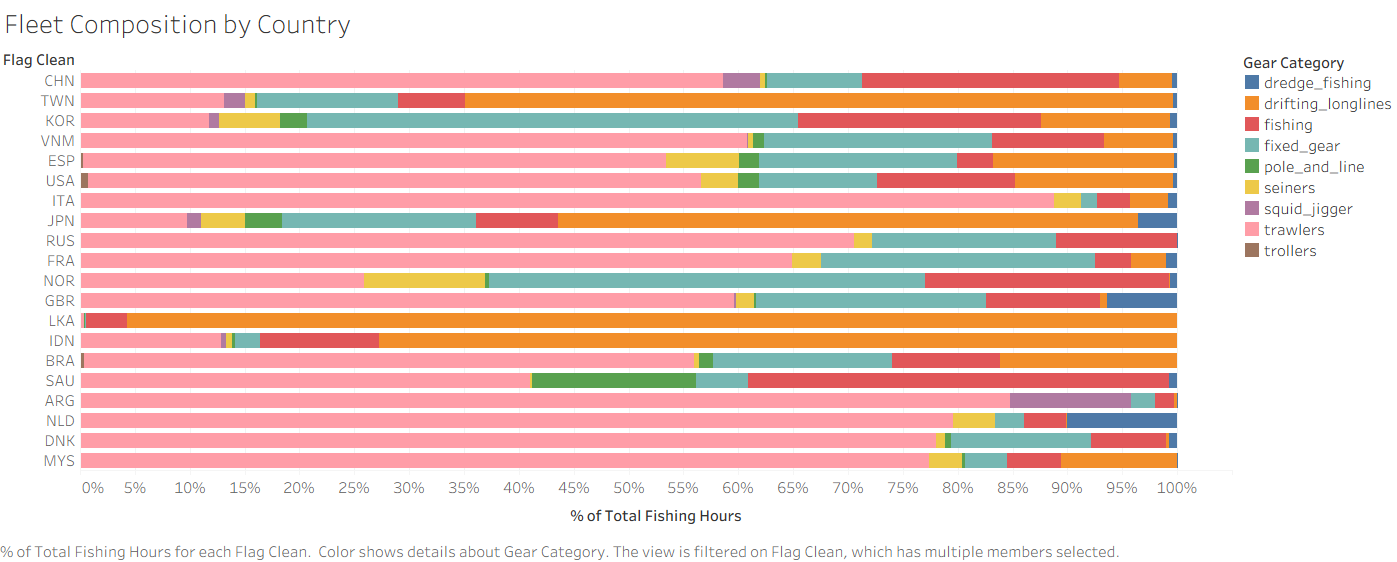
\includegraphics[width=\columnwidth]{attachments/Fleet Composition by Country.png}
  \caption{Fleet composition by country. China's fleet is notably diversified across gear types; even its modest proportional trawler share likely exceeds the total output of most other nations due to sheer fleet size. Taiwan and South Korea are dominated by drifting longlines (tuna), while Norway and France are heavily trawler-dependent.}
  \label{fig:fleet}
\end{figure}

Figure~\ref{fig:fleet} validates hypothesis~(5): fleet profiles differ sharply by flag state. China spreads effort across squid jiggers, drifting longlines, seiners and trawlers, whereas Peru is almost entirely purse seiners (anchoveta) and Vietnam is overwhelmingly trawler-dependent, implying higher bycatch risk. The chart also illustrates the scale paradox central to hypothesis~(2): a 15\% trawler share of China's fleet represents more absolute fishing hours than the entire output of most nations on the list.

\begin{figure}[h]
  \centering
  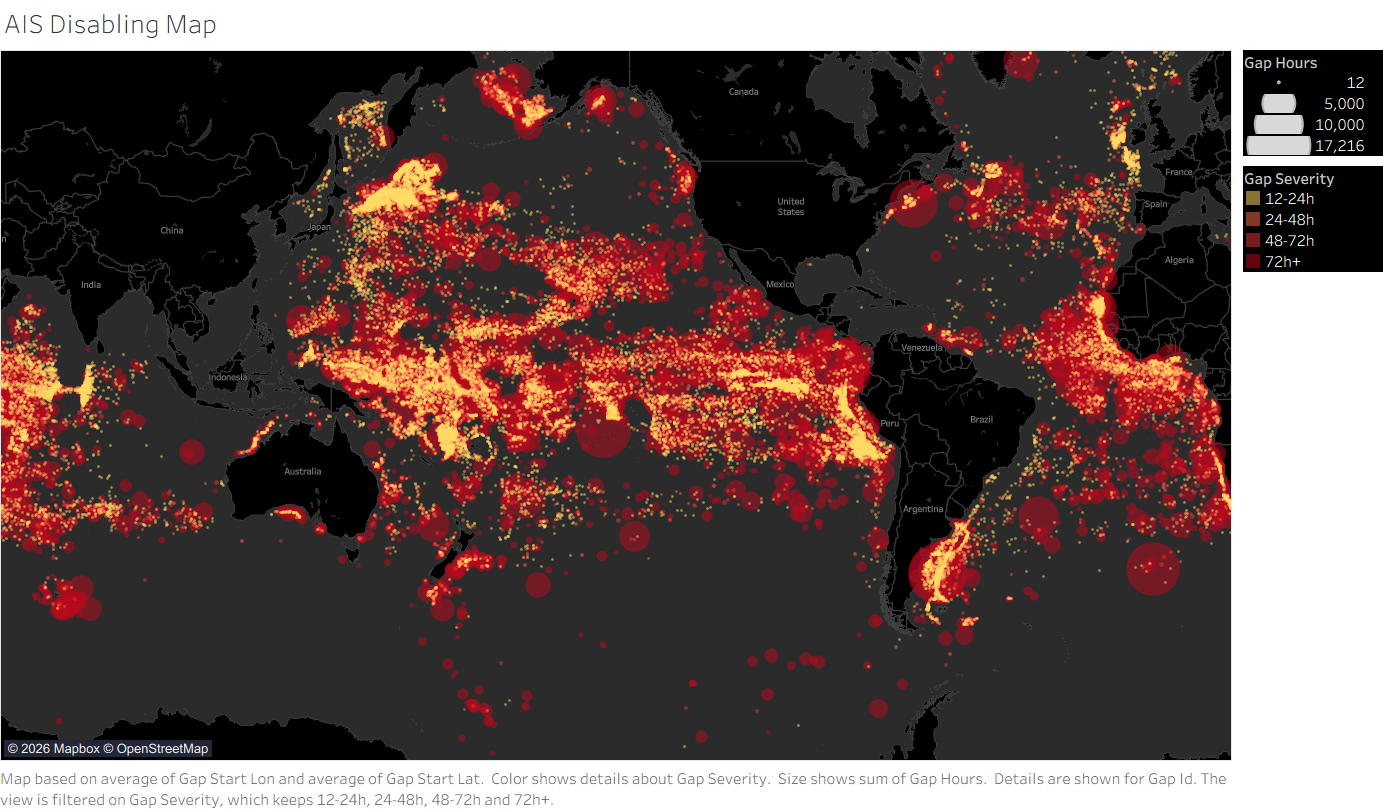
\includegraphics[width=\columnwidth]{attachments/AIS Disabling Map.png}
  \caption{AIS disabling events (2017--2019), sized by gap hours and coloured by severity. Disabling concentrates along EEZ boundaries (the Argentine shelf, West Africa, the Northwest Pacific) where high-value stocks overlap with weak enforcement.}
  \label{fig:disabling}
\end{figure}

Figure~\ref{fig:disabling} provides early support for hypothesis~(1). The largest gap-hour circles cluster on the Argentine EEZ boundary (squid jigger fleets), off West Africa where enforcement capacity is thin, and across the Northwest Pacific. Waters around Australia, Northern Europe and the US East Coast are comparatively clean, reinforcing that disabling is a behavioural choice correlated with weak enforcement rather than a satellite coverage artefact. The Southeast Asian archipelago shows dense mid-severity activity (12--24h gaps), relevant to Singapore's role as a major port state.

\subsection{Potential Unexpected Findings}
Several patterns may challenge prior assumptions: high-risk vessels may appear under developed-nation flags rather than only the usual suspects; systematic divergence between a vessel's flag state and its most-visited port may reveal flag-of-convenience behaviour; forced-labour network proximity may prove structurally broad across the global fleet; post-COVID recovery may be uneven across flag states and gear types; and GDELT news coverage may underrepresent the highest-risk regions, revealing monitoring blind spots.

\section{Project Milestones}
\begin{itemize}
    \item \textbf{Week 5} Data preparation
    \item \textbf{Week 6} Tool setup
    \item \textbf{Week 7--8} Core sheet development
    \item \textbf{Week 9--10} Dashboard assembly
    \item \textbf{Week 11} Preliminary analysis review
    \item \textbf{Week 12} Story assembly \& report drafting
    \item \textbf{Week 13} Finalisation \& presentation
\end{itemize}

\newpage
\bibliographystyle{ACM-Reference-Format}
\bibliography{sample-base}

\end{document}
\endinput
